\section{Methods}

\begin{frame}[c]{Traditional workflow:}
    \begin{overprint}
    \onslide<1>\includegraphics[scale=0.86]{imgs/workflow_trad_1.pdf}
    \onslide<2>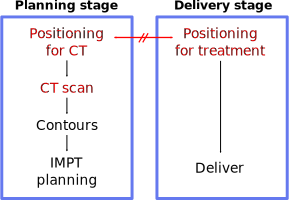
\includegraphics[scale=0.86]{imgs/workflow_trad_2.pdf}
    \end{overprint}
\end{frame}

\begin{frame}[c]{Patient cohort planned without margin around CTV}
	\begin{table}[h]
		\scalebox{0.7}{
			\begin{tabular}{ccp{1cm}|p{1cm}p{2.5cm}|p{3cm}p{3cm}}
				\hline
				Pat. No. & Location & No. beams & No. CBCTs & Plan CTV vol. ($cm^3$) & Average CTV vol. ratio (min, max) & Average CTV dice (min, max) \\
				\hline
				1 & Oropharynx & 4 & 6 & 22.3 & 1.00 (0.97, 1.05) & 0.58 (0.50, 0.67) \\
				2 & Tonsil & 2 & 6 & 9.0 & 1.02 (0.94, 1.12) & 0.87 (0.83, 0.90) \\
				3 & Oropharynx & 3 & 7 & 30.7 & 0.93 (0.90, 1.00) & 0.82 (0.77, 0.88) \\
				4 & Neck & 4 & 6 & 81.3 & 1.03 (0.98, 1.06) & 0.79 (0.75, 0.84) \\
				5 & Hypopharynx & 3 & 5 & 59.6 & 0.97 (0.95, 0.98) & 0.89 (0.87, 0.91) \\
				6 & Mouth & 3 & 7 & 116.5 & 0.78 (0.75, 0.82) & 0.87 (0.83, 0.90) \\
				7 & Larynx & 3 & 6 & 25.0 & 1.21 (1.08, 1.34) & 0.84 (0.77, 0.88) \\
				8 & Tongue & 4 & 5 & 79.9 & 1.06 (1.04, 1.11) & 0.87 (0.82, 0.91) \\
				9 & Tonsil & 2 & 6 & 12.0 & 0.98 (0.95, 1.00) & 0.87 (0.83, 0.93) \\
				10 & Oropharynx & 3 & 7 & 95.9 & 0.96 (0.91, 1.02) & 0.89 (0.85, 0.92) \\
				\hline
				Summary: & - & - & 61 & 63.22 $\pm$ 45.1 & 0.98 $\pm$ 0.11 & 0.83 $\pm$ 0.09 \\
				\hline \\
			\end{tabular}}
			\caption{Patient cohort summary}
		\end{table}
	\end{frame}

\begin{frame}[c]{What are we facing?}
    \begin{columns}[c]
        \column[c]{0.45\textwidth}
        \begin{figure}[h]
            \centering
            \includegraphics[width=\textwidth]{imgs/patient_deformation.png}
            \caption{Head and neck patient geometry changes. The arrows represent the vector field.}
        \end{figure}
        \column[c]{0.55\textwidth}
        \onslide<2>\includegraphics[width=\textwidth]{imgs/plan_evolution_V98.pdf}\\
        \onslide<2>\includegraphics[width=\textwidth]{imgs/plan_evolution_V107.pdf}
    \end{columns}
\end{frame}

\begin{frame}[c]{Traditional workflow:}
    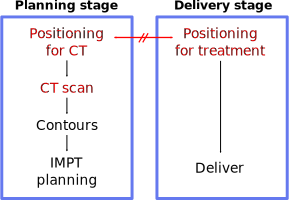
\includegraphics[scale=0.86]{imgs/workflow_trad_2.pdf}
\end{frame}

\begin{frame}[c]{Adaptation workflow:}
    \begin{overprint}
    \onslide<1>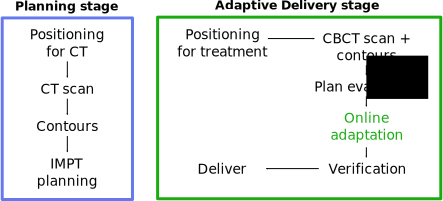
\includegraphics[scale=0.86]{imgs/workflow_adaptive_1.pdf}
    \onslide<2>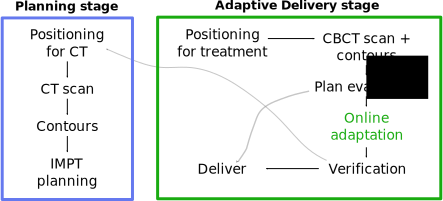
\includegraphics[scale=0.86]{imgs/workflow_adaptive_2.pdf}
    \end{overprint}
\end{frame}

\begin{frame}[c]{Necessary tools}
	\begin{columns}[t]
		\begin{column}{0.5\textwidth}
        {\setbeamercolor{block title}{bg=flame, fg=black}
        \begin{block}{Cone Beam CT (CBCT)}
            \textit{A priori} CT-based scatter correction WEPL error $< 2\%$ in head cases.\\
            {\begin{flushright}\scriptsize\textit{Park et al., Med Phys. 2015;42(8)}, \textit{Kim et al., Phys Med Bio. 2017;62(1)}\end{flushright}}
        \end{block}}
        {\setbeamercolor{block title}{bg=inchworm, fg=black}
        \begin{block}{Fast GPU MC: gPMC}
            Accurate dose calculation engine.\\
            {\hfill\scriptsize\textit{Qin et al., Phys Med Biol. 2016;61(20)}}
        \end{block}}
		\end{column}
		\begin{column}{0.5\textwidth}
			{\setbeamercolor{block title}{bg=iceberg, fg=black}
            \begin{block}{Image Registration: Plastimatch}
                Register planning CT to CBCT. Rigid and deformable (DIR), GPU B-spline\\
                {\hfill\scriptsize\textit{Shackleford et al., Phys Med Biol. 2010;55(21)}}
            \end{block}}
            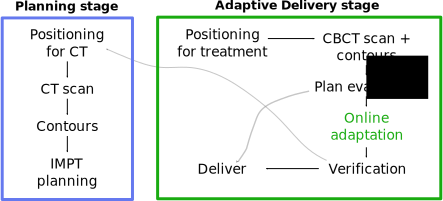
\includegraphics[width=\textwidth]{imgs/workflow_adaptive_2.pdf}
		\end{column}
	\end{columns}
\end{frame}


\begin{frame}[c]{Adaptation steps}
    Adaptation steps:
    \begin{enumerate}
        \item \textbf{Geometrical adaptation:} spots are moved following a VF and the energy is adjusted after raytracing
        \item \textbf{Weight adaptation:} tune spot weights to correct for the unbalance created by the geometrical adaptation
    \end{enumerate}
    \pause
    Why does this study not include setup uncertainties and what does it mean?
\end{frame}


\begin{frame}[c]{Geometrical adaptation: basics}
	\begin{columns}[t]
		\begin{column}{0.55\textwidth}
            Per spot $s_i = (x_0, y_0, E_0)$:
            \begin{itemize}
                \item[1:]<2-> \textbf{Raytrace} $s_i$ in CT ($r_i$)
                \item[2:]<3-> \textbf{Probe} VF at $r_i$ coords: $v_i$
                \item[3:]<4-> \textbf{Apply $v_i$ to $r_i$} coords: position where the $r_i$ should be in the CBCT
                \item[4:]<5-> \textbf{Apply $v_i$ to $s$} $\rightarrow $ $s'_i = (x_0 + \Delta v_x, y_0 + \Delta v_y, E_0)_i$
                \item[5:]<6-> \textbf{Raytrace} $s'_i$ in CBCT
                \item[6:]<7-> \textbf{Get} $\Delta E_i$
            \end{itemize}
            \only<8>{Spot adaptation: $(\Delta v_x, \Delta v_y, \Delta E)_i$}
		\end{column}
		\begin{column}{0.45\textwidth}
			\vspace{-1cm}
			\begin{figure}
                \only<1>{\includegraphics[height=0.8\textheight]{imgs/adaptation_method_0.pdf}}
                \only<2>{\includegraphics[height=0.8\textheight]{imgs/adaptation_method_1.pdf}}
				\only<3>{\includegraphics[height=0.8\textheight]{imgs/adaptation_method_2.pdf}}
				\only<4>{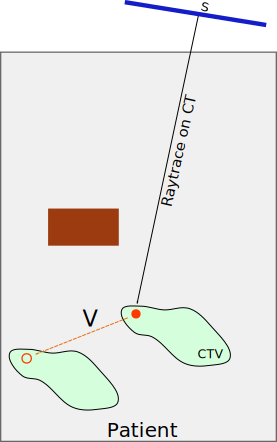
\includegraphics[height=0.8\textheight]{imgs/adaptation_method_3.pdf}}
				\only<5>{\includegraphics[height=0.8\textheight]{imgs/adaptation_method_4.pdf}}
				\only<6>{\includegraphics[height=0.8\textheight]{imgs/adaptation_method_5.pdf}}
				\only<7->{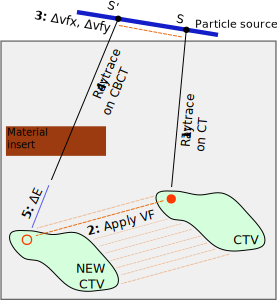
\includegraphics[height=0.8\textheight]{imgs/adaptation_method_end.pdf}}
			\end{figure}
		\end{column}
	\end{columns}
\end{frame}


\begin{frame}[c]{Geometrical adaptation: constraints}
    \begin{columns}[c]
        \begin{column}{0.45\textwidth}
            Constraints:
            \begin{itemize}
                \item {\color{brandeisblue} Free:} No constraints on spots movement $(\Delta v_x, \Delta v_y, \Delta E)_i$
                \item {\color{brandeisblue} Constrained:}
                \begin{itemize}
                    \item \textit{Couch/isocenter shift}: Average VF in the CTV
                    \item \textit{Range-shifter-of-the-day}: Average energy shift
                    \item \textit{Both}
                \end{itemize}
            \end{itemize}
        \end{column}
        \begin{column}{0.55\textwidth}
            \vspace*{-0.4cm}
            \begin{figure}[b!]
                \centering
                \includegraphics[width=\textwidth]{imgs/plan_energy_layer_destruction.pdf}\\
                \includegraphics[width=\textwidth]{imgs/plan_energy_layer_conservation.pdf}
                \caption{Distortion and conservation of plan energy layers}
            \end{figure}
        \end{column}
    \end{columns}
\end{frame}


\begin{frame}[c]{Weight tuning:}
     Taking the proposed workflow into account\ldots
	\begin{figure}[h]
		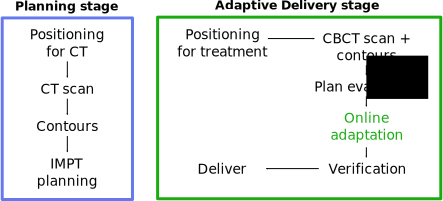
\includegraphics[scale=0.7]{imgs/workflow_adaptive_1.pdf}
	\end{figure}
    How can we gather significant information of individual spots \textbf{fast}?
\end{frame}


\begin{frame}[c]{Adaptation workflow:}
	\textbf{Use information from the initial plan: on average, 8.2\% of the spots deliver at least 50\% of the dose}
	\pause
	
	Weight tuning:
    \begin{enumerate}
    	\item Run the \textbf{geometrical adaptation} with gPMC
    	\item Define \textbf{region of interest} during simulation
    	\item Score the \textbf{dose per spot} in ROI
    	\item \textbf{Select set} of spots giving 50\% of the dose, being at least 10\% of the total spots
    	\item Accumulate adapted dose without the set
    	\item Calculate \textbf{remaining dose} for coverage in target
    	\item \textbf{Tune set weights} to fill the remaining dose with Opt4D
    \end{enumerate}
\end{frame}
